\documentclass[xcolor=pst]{beamer}
\usepackage[utf8]{inputenc}
\usepackage{ngerman}
\usepackage{beamerthemesplit}
\usepackage{epsfig}
\usepackage{tikz}
\usepackage{siunitx}
\usepackage{pbox}
\usepackage{pdfpages}
\usepackage{verbatim}
\usepackage{units}
\usepackage{algpseudocode}

\usepackage{color}
\usetheme{Antibes}
%\usepackage{multirow}

% bibliographie
\usepackage[english]{cleveref}
\usepackage[style=numeric]{biblatex}
\addbibresource{presentation.bib}
\usepackage{appendixnumberbeamer}

\usetikzlibrary{shapes.geometric, calc}

% fusszeile so aufteilen, dass autoren und titel reinpassen und seitenzahl hinzu
\setbeamertemplate{footline}
{
  \leavevmode%
  \hbox{%
  \begin{beamercolorbox}[wd=.6\paperwidth,ht=2.25ex,dp=1ex,center]{author in head/foot}%
    \usebeamerfont{author in head/foot}\insertshortauthor
  \end{beamercolorbox}%
  \begin{beamercolorbox}[wd=.4\paperwidth,ht=2.25ex,dp=1ex,center]{title in head/foot}%
    \usebeamerfont{title in head/foot}\insertshorttitle\hspace*{2.5em}\insertframenumber
  \end{beamercolorbox}}%
  \vskip0pt%
}

% keine navigationssymbole in der fusszeile
\beamertemplatenavigationsymbolsempty

% so definiert man neue makros
\newcommand{\IFF}{\Leftrightarrow}
\newcommand{\todo}[1]{\textbf{\color{red}todo:\color{black}#1}}

\author{
  Lukas Götz, Stefan Dang \& Dorle Osterode
}
\title{Gt-Scaffolder: TODO}
\institute[FBI - UniHH]{Universität Hamburg - Fachbereich Bioinformatik}
\date{2015-01-30}

\subject{}
\keywords{}

\begin{document}
\begin{frame}[plain]
\titlepage
\end{frame}

% keine seitenzahl auf der inhaltsangabe zeigen (theme nur fuer diese folie anpassen)
\bgroup
\makeatletter
\setbeamertemplate{footline}
{
  \leavevmode%
  \hbox{%
  \begin{beamercolorbox}[wd=.6\paperwidth,ht=2.25ex,dp=1ex,center]{author in head/foot}%
    \usebeamerfont{author in head/foot}\insertshortauthor
  \end{beamercolorbox}%
  \begin{beamercolorbox}[wd=.4\paperwidth,ht=2.25ex,dp=1ex,center]{title in head/foot}%
    \usebeamerfont{title in head/foot}\insertshorttitle\hspace*{2.5em}
  \end{beamercolorbox}}%
  \vskip0pt%
}
\makeatother
\begin{frame}{Übersicht}
\tableofcontents
\end{frame}
\egroup % ab hier das normale theme weiterverwenden


\section{Motivation}
\begin{frame}
\setcounter{framenumber}{1}
  \frametitle{Einführung}

  \begin{columns}
    \begin{column}{.45\textwidth}
      \begin{itemize}
      \item ungleichmäßige Coverage \& Wiederholungen $\rightarrow$
         (Contigs)
      \item Contigs werden zu Abschnitten angeordnet (Scaffolds)
      \end{itemize}
    \end{column}
    \begin{column}{.45\textwidth}
      \begin{center}
        \begin{figure}[t]
          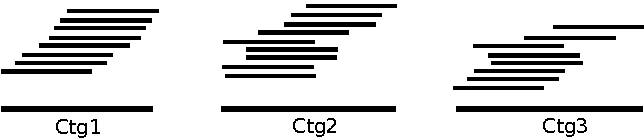
\includegraphics[width=\textwidth,height=0.8\textheight,keepaspectratio]{figures/Scaffolding.pdf}
        \end{figure}
        \begin{figure}[t]
          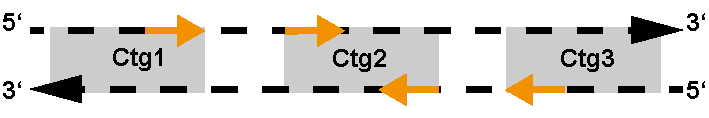
\includegraphics[width=\textwidth,height=0.8\textheight,keepaspectratio]{figures/Scaffolding_2.pdf}
        \end{figure}
      \end{center}
    \end{column}
  \end{columns}
\end{frame}

\begin{frame}
  \frametitle{Einführung}
  \begin{itemize}
  \item Verwendung der Read-Paar Informationen:
    \begin{itemize}
    \item Fragmentgröße
    \item Position auf Contigs
    \end{itemize}
  \item Read-Paare stammen aus paired-end oder mate-pair Sequenzierung
  \end{itemize}
\end{frame}

\begin{frame}
  \frametitle{Scaffolding Problem}
  \begin{center}
    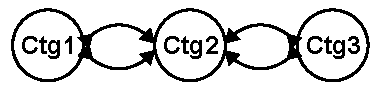
\includegraphics[width=0.5\textwidth,height=0.8\textheight,keepaspectratio]{figures/Scaffolding_3.pdf}
  \end{center}
  \begin{itemize}
  \item Scaffold Graph:
    \begin{itemize}
    \item Knoten entsprechen Contigs
    \item Kanten beschreiben Read-Paar
      Informationen
    \item bidirektionaler Graph
    \end{itemize}
  \item Scaffolding ist NP-vollständig
  \item Strategie: Zerlegung in
    Teilprobleme, die unabhängig voneinander gelöst werden
  %% \item Beschreibung des Scaffolding Problems mit Hilfe eines
  %%   Graphen (Scaffold Graph), wobei deren Zusammenhangskomponenten
  %%   Teilprobleme darstellen
    %hier Scaffolding_3.svg
  \end{itemize}
\end{frame}

\section{Methoden}
\begin{frame}
  \frametitle{Allgemein}
  \begin{itemize}
  \item Reimplementation der Scaffolding Methode von SGA (C++) im
    Rahmen von Genometools (C)
  \item basiert auf Konstruktion eines Graphen über die Beziehungen
    zwischen Contigs (Scaffold Graph)
  \end{itemize}
\end{frame}

\begin{frame}
  \frametitle{Gt-Scaffolder}
  \begin{itemize}
  \item Eingabe:
    \begin{itemize}
    \item Contigs
    \item Distanzinformationen
    \item Astatistik %spelling?
    \end{itemize}
  \item Ausgabe:
    \begin{itemize}
    \item Scaffolds
    \item (rekonstruierte Sequenzen)
    \end{itemize}
  \end{itemize}
\end{frame}

\begin{frame}
  \frametitle{Übersicht der Schritte}
  \begin{itemize}
  \item Konstruktion des Scaffold Graph:
    \begin{itemize}
    \item nicht-repetitive Contigs als Knoten
    \item bidirektionalen Kanten zwischen Contigs
    \end{itemize}
  \item Filterung des Graphen:
    \begin{itemize}
    \item inkonsistente Kanten
    \item polymorphe Knoten
    \item Zyklen
    \end{itemize}
  \item Ermittlung aller Zusammenhangskomponenten
  \item Bestimmung des Pfades mit größter Sequenzabdeckung für jede
    Zusammenhangskomponente
  \end{itemize}
\end{frame}

\section{Ergebnisse}
\begin{frame}
  \frametitle{Vergleich mit SGA}

\end{frame}

\section{Diskussion und Ausblick}
\begin{frame}
  \frametitle{Diskussion}
  \begin{itemize}
  \item Gründe für neue Implementation
    \begin{itemize}
    \item geringerer Speicherplatzverbrauch, schnellere Laufzeit
       für Gt-Scaffolder (C-Implementation) im Vergleich zu
       SGA-Scaffolder (C++ Implementation) bei gleicher Güte
       der Ergebnisse (quod esset demonstrandum)
    \item geringere Abhängigkeit von fremder Software, Einbau
      von Abyss DistEst in Gt-Scaffolder (zur Ermittlung der
      Read-Paar Informationen) und Berechnung der A-Statistik
      durch Read-Joiner anstelle von Pysam
    \end{itemize}
  \end{itemize}
\end{frame}

\begin{frame}
  \frametitle{Ausblick}
  \begin{itemize}
  \item was wir noch alles machen muessen (kann erst am ende
    ausgefuellt werden)
  \end{itemize}
\end{frame}


\appendix
\section*{Bibliographie}
\begin{frame}{Bibliographie}
    %\nocite{Hernandez:2014jp, Hernandez:2008jw}
    \printbibliography
\end{frame}
\end{document}
